\documentclass[a4paper,12pt]{article}
\usepackage[colorlinks=false,pdfborder=000]{hyperref}
\usepackage{enumerate}
\usepackage{multirow}
\usepackage{titling}
\usepackage[top=1.2in, bottom=1.2in, left=1.2in, right=1.2in]{geometry}
\usepackage[dvips]{graphicx,color}
\usepackage{times}
\usepackage{comment}
\usepackage{subfigure}
\usepackage{amssymb}
%%%%%%%%%%%%%%%%%%%%%%%%%%%%%%%%%%%%%%%%%%%%%%%%%%%%%%%%%%%%%%%%%%%%%%%%%%%%%%%%%%%%%%%%%%%%%%%%%%%%%%%%%%%%%%%%%%%%%%%%%%%%
\newcommand{\CSE}{\href{http://www.cse.cuhk.edu.hk}{Department of Computer Science and
Engineering}}
\newcommand{\CUHK}{\href{http://www.cuhk.edu.hk}{The Chinese University of Hong Kong}}
\newcommand{\mymail}{\mbox{\textcolor{blue}{\underline{zgxiao@cse.cuhk.edu.hk}}}}
\newcommand{\myname}{\href{http://www.cse.cuhk.edu.hk/~zgxiao}{XIAO Zigang}}
\newcommand{\header}[1]{\noindent {\bf \\#1\\}}
\newcommand{\NE}{Nash Equilibrium }
\newcommand{\tot}{\frac{2}{3}}
%%%%%%%%%%%%%%%%%%%%%%%%%%%%%%%%%%%%%%%%%%%%%%%%%%%%%%%%%%%%%%%%%%

% modify the font size of title, author and date
\pretitle{\begin{center}\bf \LARGE} \posttitle{\par\end{center}}
\preauthor{\begin{center}
            \small \lineskip 0.5em%
            \begin{tabular}[t]{c}}
\postauthor{\end{tabular}\par\end{center}}
\predate{\begin{center}\small} \postdate{\par\end{center}}

\title{CSC 5350 Assignment 2}
\author{\myname\\\mymail\\\CSE\\\CUHK}
\date{\today}
%%%%%%%%%%%%%%%%%%%%%%%%%%%%%%%%%%%%%%%%%%%%%%%%%%%%%%%%%%%%%%%%%%
\begin{document}
\maketitle
%\begin{pspicture}(-0.5,0)(2.5,1)
%\psdots(0,0)(2,0)(1,1)
%\end{pspicture}
\begin{enumerate}
%%%%%%%%%%%%%%%%%%%%%%%%%%%%%%%%%%%%%%%%%%%%%%%%%%%%%%%%%%%%%%%%%%
%%%%%%%% 1
\item
The game $\Gamma$ is given in Figure \ref{fig:deviate}.There is only one player, player 1, 
and the payoff of the infinite history is 2.
We verify whether $s^*=(aaa\ldots)$ is a subgame perfect equilibirum.

In the subgame $\Gamma(\varnothing)$, by switching the action to $b$, 
we get the strategy $s_1=(baa\ldots)$, in which the payoff is 1. 
We have $O(s^*) \succsim_1 O(s_1)$.

Similar case happens in the subgame $\Gamma(b)$. We have $s_2=(aba\ldots)$ and $O(s^*) \succsim_1 O(s_3)$.
We can find out $s^*$ satisfies the requirement to be a subgame perfect equilibirum in \textit{one derivation property}.

However, by changing strategy to $(bbb\ldots)$, we get payoff 2,which is better than $s^*$.
The one deviation property does not hold.

\begin{figure}[!ht]
\centering
	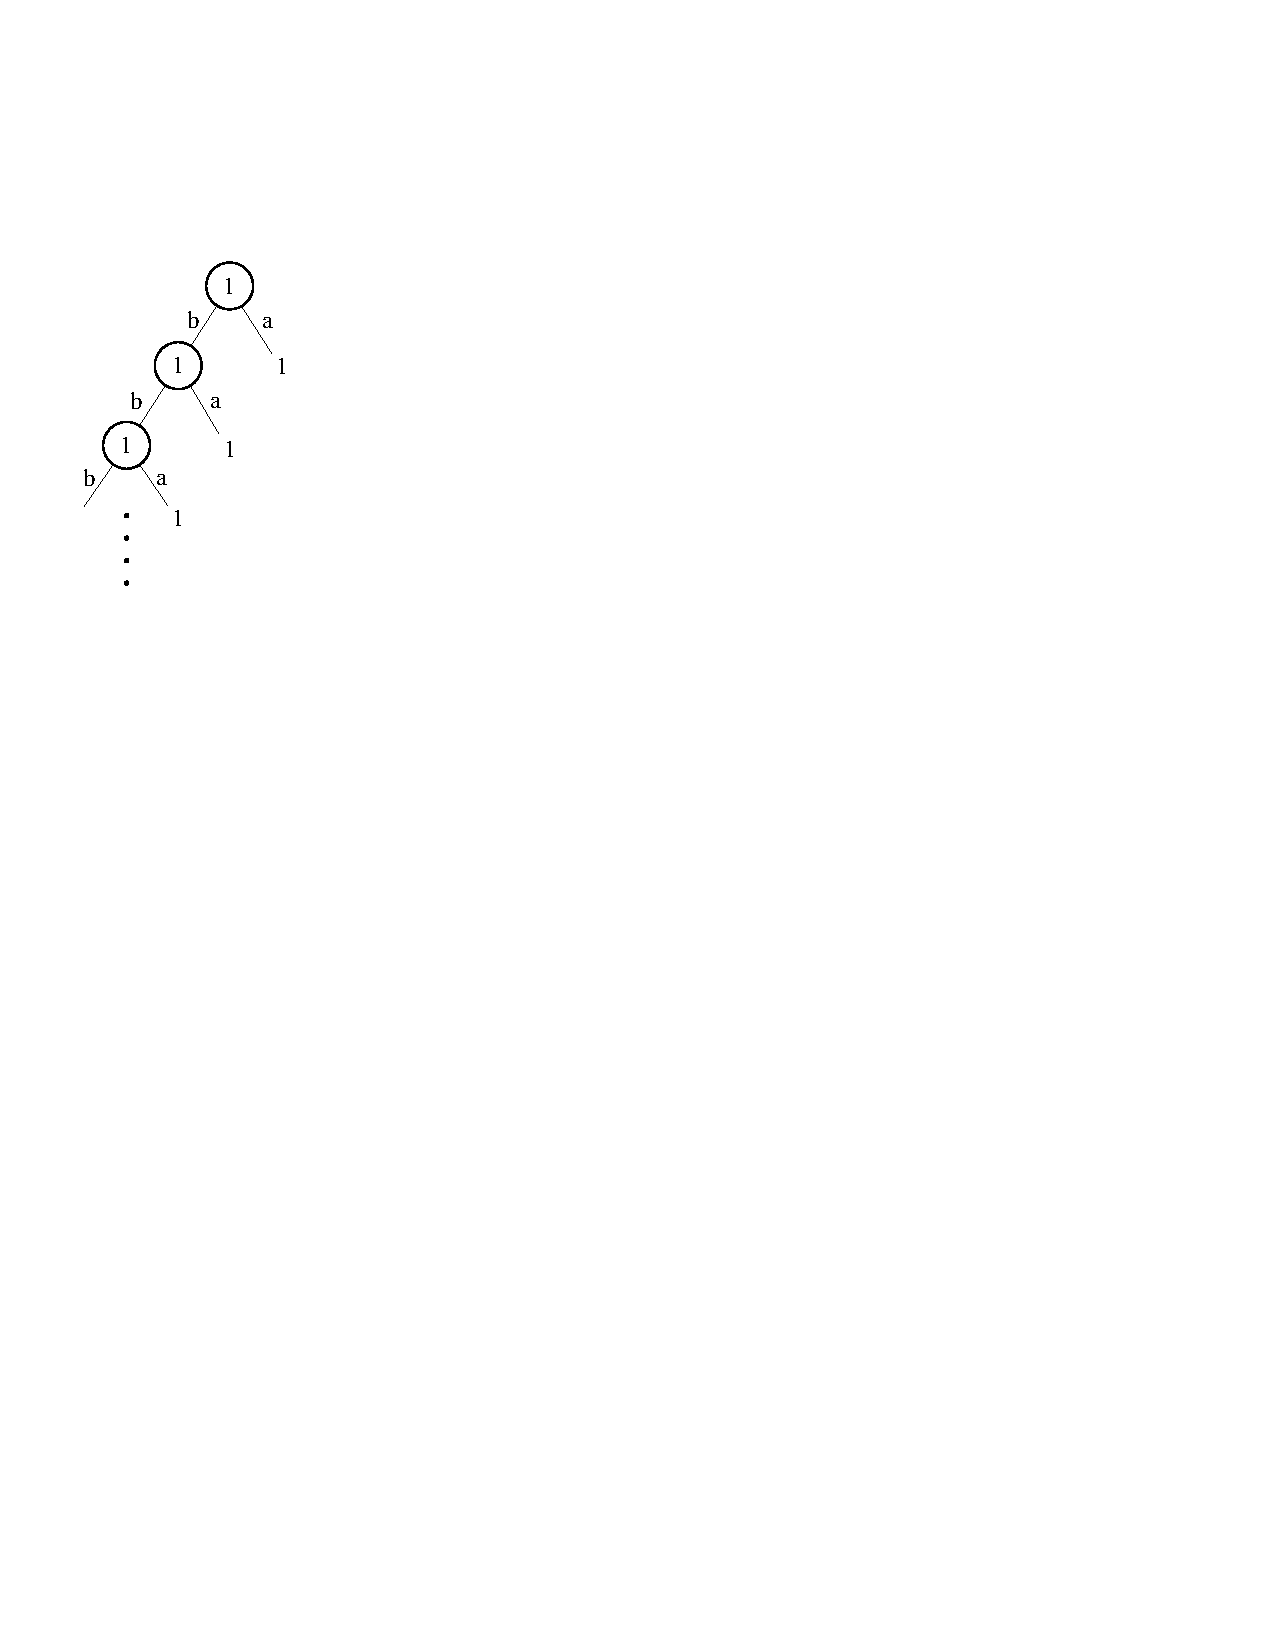
\includegraphics[width=0.2\textwidth]{deviate.pdf}
	\caption{An extensive game with infinite horizon}
	\label{fig:deviate}
\end{figure}

%%%%%%%%%%%%%%%%%%%%%%%%%%%%%%%%%%%%%%%%%%%%%%%%%%%%%%%%%%%%%%%%%%
%%%%%%%% 2
\item
Let the length of the subgame be $l$. 

When $l=1$, it is trivial that for the player who plays the only move in this game, 
the outcomes are the same if \textit{no indifference condition} holds. 

Suppose for $l=k$ the statement is true.
When $l=k+1$, i.e. the length of the current subgame $\Gamma(h)$ is $k+1$,
let $P(h)=i$. For all actions $a \in A(h)$,let $O(h,a)$ be the outcome of subgame $\Gamma(h,a)$. 
For any two action $a_1$ and $a_2$ in $A(h)$, 
if they are the actions player $i$ has to take to achieve Nash Equilibrium,
the payoff of the outcomes induced by them should be the same
(note that the extensive game is finite horizon,
thus we only have to verify the strategy induced by changing the action after initial history of $\Gamma(h)$).
By hypothesis we know that all outcomes are equivalent in a subgame $\Gamma(h,a)$,
hence player i will be indifferent in both subgame perfect equilibrium.
Then we proved that all players are indifferent among all subgame perfect equilibrium outcomes of $\Gamma(h)$.


According to the one deviation property of finite extensive game, 
we know that for every subgame $\Gamma(h)$, 
we only have to consider the current action player $i=P(h)$ will take to verify whether strategy $s''$ is nash equilibrium.
We know from first part of this exercise that in each subgame, 
the player would be indifferent among all subgame perfect nash equilibrium outcome, which means if $s$ and $s'$
are both subgame perfect equilibrium, player $i'$s strategy $s_i$ and $s'_i$ should leads to the same outcome at each subgame,
and it is still subgame perfect equilibrium.
Then we know that we could actually construct a strategy profile from $s$ and $s'$ by setting every player $i'$s strategy to 
either $s_i$ or $s'_i$. 
So any strategy profile $s''$ in which for each player $i$ the strategy $s''_i$ 
is equal to either $s_i$ or $s'_i$ is a subgame perfect equilibrium.


%%%%%%%%%%%%%%%%%%%%%%%%%%%%%%%%%%%%%%%%%%%%%%%%%%%%%%%%%%%%%%%%%%
%%%%%%%% 3
\item
Formulate the game as $\Gamma=\langle N,H,P,(\succsim_i)\rangle$,where
\begin{itemize}
\item $N=\{1,2,3\}$
\item $H=\{\varnothing\} \cup D \cup \{(d,a):d \in D,a \in A \times A\}$, \\
where $D=\{(d_1,d_2,d_3)|d_1,d_2,d_3 \in R^+, \Sigma_{i=1}^3 d_i=1\}$ and
$A=\{yes,no\}$
\item $P(\varnothing)=1, P(d)=\{2,3\}$, where $d \in D$
\item
For each $i \in N$ we have preference relation as follows:
\begin{itemize}
\item[-]
if $d_i > d'_i, (d,(yes,yes))\succ_i(d',(yes,yes))$
\item[-]
if $d_i=0, (d,(yes,yes))\sim_i (d,a)$\\where $a \in \{yes,no\} \times \{yes,no\}$
\item[-]
if $d_i>0, (d,(yes,yes))\succ_i(d,a)$, where $a\neq (yes,yes)$
\item[-]
if $a\neq (yes,yes)$ and $b\neq (yes,yes)$,\\for any $d,d'\in~D, (d,a)~\sim_i~(d',b)$
\end{itemize}
\end{itemize}

\begin{figure}[!ht]
\centering
\includegraphics[width=0.4\textwidth]{pie.pdf}
\caption{Illustration of the game}
\label{fig:pie}
\end{figure}

Figure \ref{fig:pie} illustrate some part of the game. 
We can assign some value to the terminal history as the outcome which satisfies the preference relation as in Figure \ref{fig:pie}.

In each subgame $\Gamma(h)$ where $h=(d)$,we can identify their Nash Equilibrium.
\begin{enumerate}[(1)]
\item
If both of player $2$ and $3$ choose $yes$ for any $d \in D$ player $1$ proposes, 
$(d,(yes,yes))$ is a Nash Equilibrium.
By both choosing $yes$, player $2$ and $3$ get $d_2$ and $d_3$ respectively and none of them get better if deviates.
\item 
If either one or both of them DO NOT choose $yes$, suppose player $1$ proposes a division $d$,
\begin{itemize}
	\item if $d_2>0,d_3>0$, $(no,no)$ is the only equilibrium.
	\item if $d_2=0,d_3>0$, $(no,no),(no,yes)$ are equilibrium.
	\item if $d_2>0,d_3=0$, $(no,no),(yes,no)$ are equilibrium.
	\item if $d_2=0,d_3=0$, $(no,no),(no,yes),(yes,no)$ are equilibrium.
\end{itemize}
\end{enumerate}

Then we verify the equilibirum in the entire game.

First we note that a strategy of player 2 \& 3 are responses to all possible value of $d\in D$,
e.g. $\{(0.5,0.25,0.25)\mapsto(yes,yes),(1,0,0)\mapsto(yes,no),...\}$ .
A strategy of player 1 is a proposal of division $d$, e.g. $\{ \varnothing \mapsto (0,1,0) \}$,$\{ \varnothing \mapsto (0.1,0.5,0.4) \}$.
Thus a strategy profile is $s=(d,a)$ where $d$ and $a$ is a strategy of player 1 and player 2 \& 3, respectively.
Then we can identify two types of subgame perfect equilibrium.
\begin{itemize}
  \item
For some $d \in D$ with $d_1>0$, if player 2 \& 3 respond $(yes,yes)$,
player 1 can get $d_1$ and he can make best by deviating to $d^*$ where $d_1^* \ge d$ for all $d$ in $(d,(yes,yes))$.
This is a subgame perfect equilibrium since we have proved in $(1)$ that
any $(yes,yes)$ induced by the strategy profile $(d,\{e\mapsto(yes,yes):e\in D\})$ are equilibrium in
the subgame following the history player 1 propose a division $d$.

  \item
For all $d\in D$ with $d_1>0$, player 2 \& 3 do not respond $(yes,yes)$,
and for all situation listed in $(2)$ player 2 \& 3 respond accordingly
by choosing one of the strategy given in that particular situation,
it is subgame perfect for any $d\in D$ that player 1 can choose,
since all the players always get nothing in the outcomes of these strategy profiles,
no matter one deviates or not.
\end{itemize}

%%%%%%%%%%%%%%%%%%%%%%%%%%%%%%%%%%%%%%%%%%%%%%%%%%%%%%%%%%%%%%%%%%
%%%%%%%% 4
\item
\begin{enumerate}[a.]
\item
Let $k_t$ be the opponent of player $1$ in period $t$.
The payoff of $k_t$ is the sum of payoff he will get in period $t$.
When player $1$ sticks to $D$ in a round,
he can not get better payoff because by deviating he gets 0 in that round.
Also for each subgame in which a period $t$ starts,
$k_t$ only cares his living period $t$, i.e. he wants to maximize payoff in $t$.
Hence for each period $t$ by choosing $D$ for each player $k_t$ it is subgame perfect.

The payoff of player $1$ is $\Sigma_{\gamma}\Sigma_{a\in A}\frac{\beta_a}{\gamma}u_i(a)$.
If his opponent always chooses $D$, 
he cannot get better because by deviating he gets 0 in a particular round.

In all,the subgame perfect equilibrium of this game is unique. Player $1$ chooses $D$ in
each period and the other player chooses $D$.

\item
Consider the Modified Prisoner's Dilemma Game, when Player $1$ chooses $C$,
Player $2$ would choose $C$.
When Player $1$ chooses $D$, Player $2$ would choose $D$.
In order to maximize what $k_t$ can get in a period $t$,
ideally he should choose whatever player $1$ chooses.
Then the possible strategy for each round should be $(C,C)$ or $(D,D)$.
Also it is true for player $1$.

\begin{table}[!ht]
\centering
    \begin{tabular}{|c|c|c|}
    \hline
      & C     & D     \\\hline
    C & (3,3) & (0,0) \\\hline
    D & (5,0) & (1,1) \\\hline
    \end{tabular}
    \caption{Modified Prisoner's Dilemma}
\end{table}

Suppose there is a series of outcomes consists of $(C,C)$ and $(D,D)$,
e.g. 
\begin{displaymath}
((C,C),(D,D),(D,D),(C,C),(D,D))	
\end{displaymath}
Then for each player he should stick to this pattern,
and it is possible for player $1'$s opponent to do so because he is \textit{informed of the actions take in every previous period}.
Player $k_t$ would not deviate unless player 1 deviates,since he could not make better by deviating.
However player 1 might deviate by changing from $C$ to $D$ in $(C,C)$,
$k_t$ should choose $(D,D)$ in the subsequent game, so does player 1.
This is the subgame perfect equilibrium.

In this equilibrium, we can see that the average payoff of player 1 should be $(3i+j)/(i+j)$,
where $i,j$ is the number of $(C,C)$ and $(D,D)$, respectively. Because 
\begin{displaymath}
x=\frac{3i+j}{i+j}=1+\frac{2}{1+\frac{j}{i}}
\end{displaymath}
We get $\max x=3 $ when $j=0$; $\min x=1$ when $\frac{j}{i}\rightarrow \infty$.
Also, if one deviates, the subsequent outcomes would be $(D,D)$ forever.
Then the average payoff of player 1 will also be 1,too.
Hence we proved that $x\in[1,3]$ under the strategy proposed, which is a subgame perfect equilibrium,
i.e. there is a subgame perfect equilibrium in which player $1'$s average payoff is $x$.

\end{enumerate}
%%%%%%%%%%%%%%%%%%%%%%%%%%%%%%%%%%%%%%%%%%%%%%%%%%%%%%%%%%%%%%%%%%
\end{enumerate}

~\\*
\center{\textbf{--- End of Assignment---}}
\end{document}
